Plot the position of the CG and the contact point on the same plot for the range $0 \leq \phi \leq \frac{\pi}{4}$. What do you notice?

\begin{solution} \
\begin{lstlisting}
phi = [0:0.1:pi/4];
x_cg = r * phi - (r - ybar)*sin(phi);
y_cg = r - (r - ybar)*cos(phi);
x_cp = r * phi;
y_cp = zeros(size(phi));
plot(x_cg, y_cg, 'bx', x_cp, y_cp, 'rx')
axis equal
\end{lstlisting}

\begin{center}
    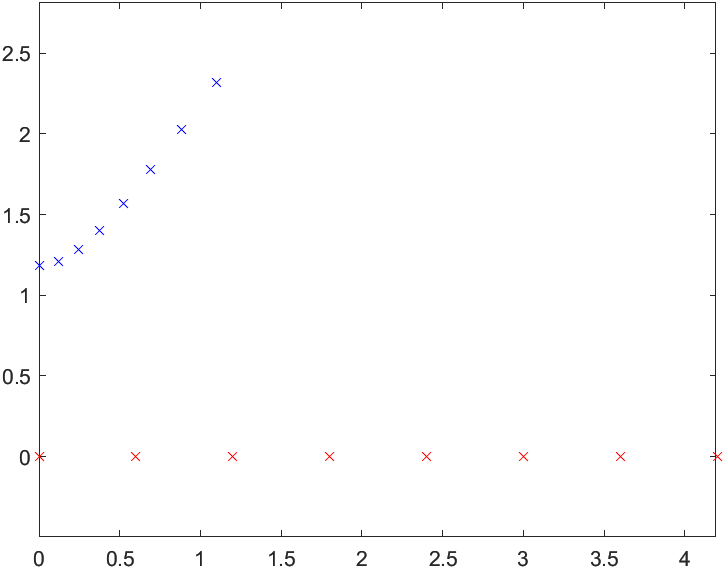
\includegraphics[width=0.5\textwidth]{img/e3p3.png}
\end{center}

The center of gravity is always closer to $0$ in the $\hat{x}$ direction.
\end{solution}